% !TEX program = xelatex
% =====================================================================================================================
%  LABORATORY REPORT  ·  Laurevine Plum template
%  Fonts: TeX Gyre Termes (body, bundled) + TeX Gyre Heros (headings/tables, falls back to bundled Arimo).
%  Edit the clearly marked blocks in the preamble; the body only needs your content.
%  Text shown in amber via \ph{...} is replaceable placeholder content. All numbers are SAMPLE data (pendulum / g).
% =====================================================================================================================
\documentclass[12pt,a4paper]{article}

% ---- Fonts -----------------------------------------------------------------------------------------------------------
% CUSTOMIZE: body font = \setmainfont (Design > Fonts > Body). Heading font = \lpHeadingFont (Design > Fonts > Heading);
% it is also used for table headers, captions, boxes and the page header. TeX Gyre Heros is used when installed,
% otherwise the bundled Arimo (a Helvetica-style sans) takes its place.
\usepackage{fontspec}
\setmainfont{TeX Gyre Termes}
\IfFontExistsTF{TeX Gyre Heros}{%
  \newfontfamily\lpHeadingFont{TeX Gyre Heros}%
}{%
  \newfontfamily\lpHeadingFont{Arimo}%
}

% ---- Mathematics -----------------------------------------------------------------------------------------------------
% Termes Math matches the body text when available; otherwise the default Latin Modern maths is kept.
\usepackage{amsmath}
\IfFontExistsTF{TeX Gyre Termes Math}{%
  \usepackage{unicode-math}%
  \setmathfont{TeX Gyre Termes Math}%
}{}

% ---- Page layout and spacing -------------------------------------------------------------------------------------------
% CUSTOMIZE: margins (Layout > Geometry), line spacing (\setstretch), paragraph spacing (\parskip).
\usepackage[a4paper,margin=2.5cm]{geometry}
\usepackage{microtype}
\usepackage{setspace}
\setstretch{1.08}
\setlength{\parindent}{0pt}
\setlength{\parskip}{0.5em plus 0.15em minus 0.1em}
\setlength{\headheight}{15pt}
\widowpenalty=10000 \clubpenalty=10000

% ---- Colors ------------------------------------------------------------------------------------------------------------
% CUSTOMIZE: restrained scientific palette (Design > Theme colors edits the lp* names below).
\usepackage[table]{xcolor}
\definecolor{lpBody}{HTML}{1E2A35}          % body text
\definecolor{lpAccent}{HTML}{1F4E79}        % links, caption labels, boxes, plot data
\definecolor{lpAccent2}{HTML}{B04A2F}       % secondary colour (fit lines, second data series)
\definecolor{lpSection}{HTML}{1F4E79}       % \section
\definecolor{lpSubsection}{HTML}{2C6B6F}    % \subsection
\definecolor{lpSubsubsection}{HTML}{4A5A6A} % \subsubsection
\definecolor{lpMuted}{HTML}{5F6F7E}         % header/footer, labels
\definecolor{lpRule}{HTML}{9FB1C1}          % rules and borders
\definecolor{lpGrid}{HTML}{D5DDE5}          % plot grid
\definecolor{lpPanel}{HTML}{F1F5F9}         % light panel background
\definecolor{lpTableHead}{HTML}{DCE6EF}     % table header row
\definecolor{lpCaution}{HTML}{A63D2F}       % safety notes
\definecolor{lpCautionBG}{HTML}{FBF0EE}
\definecolor{lpPlaceholder}{HTML}{8C6D1F}   % replaceable placeholder text
\AtBeginDocument{\color{lpBody}}

% Placeholder text. To switch the amber highlight off in the final report: \renewcommand{\ph}[1]{#1}
\newcommand{\ph}[1]{\textcolor{lpPlaceholder}{#1}}

% ---- Packages ----------------------------------------------------------------------------------------------------------
\usepackage{graphicx}
\usepackage{array}
\usepackage{booktabs}
\usepackage{float}
\usepackage{enumitem}
\usepackage{siunitx}
\usepackage{sectsty}
\usepackage{fancyhdr}
\usepackage{caption}
\usepackage{tcolorbox}
\tcbuselibrary{skins,breakable}
\usepackage{pgfplots}
\pgfplotsset{compat=1.17}

% Units: write \SI{9.81}{\metre\per\second\squared} or \si{\metre}; \num{...} for plain numbers.
\sisetup{per-mode=symbol, exponent-product=\cdot}

% ---- Headings ----------------------------------------------------------------------------------------------------------
% CUSTOMIZE: heading font and colours (Design > Fonts / Theme colors / Heading design).
\sectionfont{\lpHeadingFont\color{lpSection}}
\subsectionfont{\lpHeadingFont\color{lpSubsection}}
\subsubsectionfont{\lpHeadingFont\color{lpSubsubsection}}

% ---- Lists -------------------------------------------------------------------------------------------------------------
\setlist{itemsep=0.15em, topsep=0.25em, parsep=0pt}
\setlist[itemize,1]{label={\textcolor{lpAccent}{\textbullet}}, leftmargin=1.6em}
\setlist[enumerate,1]{label={\textcolor{lpAccent}{\arabic*.}}, leftmargin=1.8em}

% ---- Captions ----------------------------------------------------------------------------------------------------------
% Table captions go above the table, figure captions below.
\DeclareCaptionFont{lpAccentFont}{\color{lpAccent}}
\DeclareCaptionFont{lpHeadFont}{\lpHeadingFont}
\captionsetup{font=small, labelfont={lpHeadFont,bf,lpAccentFont}, labelsep=period, format=hang,
              justification=raggedright, singlelinecheck=false, skip=6pt}
\captionsetup[table]{position=top}

% ---- Tables ------------------------------------------------------------------------------------------------------------
% Usage inside a table: \tblsetup, then \toprule\rowcolor{lpTableHead} {\hdr{Header / unit}} & ... \\ \midrule ... \bottomrule
% (wrap headers of siunitx S columns in an extra pair of braces, as in the examples).
\newcommand{\tblsetup}{\small\renewcommand{\arraystretch}{1.22}\arrayrulecolor{lpRule}}
\newcommand{\hdr}[1]{{\lpHeadingFont\bfseries\footnotesize #1}}
\newcommand{\tblnote}[1]{\par\smallskip{\footnotesize\raggedright\textit{Note.}\ #1\par}}

% ---- Highlight boxes ---------------------------------------------------------------------------------------------------
% \begin{keyresult}...\end{keyresult}  highlights a headline result
% \begin{labnote}...\end{labnote}      neutral remark       \begin{caution}...\end{caution}  safety warning
% \begin{samplecalc}[Title]...\end{samplecalc}  framed worked calculation
\newcommand{\boxlabel}[2][lpAccent]{{\lpHeadingFont\bfseries\small\color{#1}#2.}\ }
\tcbset{lpbase/.style={enhanced, breakable, sharp corners, frame hidden, boxrule=0pt,
  left=8pt, right=8pt, top=5pt, bottom=5pt, before skip=8pt, after skip=8pt}}
\newtcolorbox{keyresult}{lpbase, colback=lpPanel, borderline west={2pt}{0pt}{lpAccent},
  before upper={\boxlabel{Key result}}}
\newtcolorbox{labnote}{lpbase, colback=lpPanel, borderline west={2pt}{0pt}{lpRule},
  before upper={\boxlabel[lpMuted]{Note}}}
\newtcolorbox{caution}{lpbase, colback=lpCautionBG, borderline west={2pt}{0pt}{lpCaution},
  before upper={\boxlabel[lpCaution]{Safety}}}
\newtcolorbox{samplecalc}[1][Sample calculation]{enhanced, breakable, sharp corners, colback=white,
  colframe=lpRule, boxrule=0.4pt, colbacktitle=lpPanel, coltitle=lpAccent,
  fonttitle=\lpHeadingFont\bfseries\small, left=8pt, right=8pt, top=4pt, bottom=4pt,
  toptitle=3pt, bottomtitle=3pt, before skip=8pt, after skip=8pt, title={#1}}

% ---- Plots (pgfplots) --------------------------------------------------------------------------------------------------
\pgfplotsset{lpaxis/.style={width=0.86\linewidth, height=7.2cm, grid=major,
  grid style={draw=lpGrid, line width=0.3pt}, axis line style={draw=lpMuted}, tick style={draw=lpMuted},
  tick label style={font=\footnotesize}, label style={font=\small},
  legend style={font=\footnotesize, draw=lpRule, fill=white, fill opacity=0.9, text opacity=1,
                at={(0.03,0.97)}, anchor=north west}, legend cell align=left}}

% ---- Header and footer -------------------------------------------------------------------------------------------------
% CUSTOMIZE: running header text is set in the REPORT DETAILS block below (Layout > Header and footer also works).
\pagestyle{fancy}
\fancyhf{}
\renewcommand{\headrulewidth}{0.4pt}
\renewcommand{\headrule}{{\color{lpRule}\hrule width\headwidth height\headrulewidth}}
\fancyhead[L]{\lpHeadingFont\footnotesize\color{lpMuted}\LabShortTitle}
\fancyhead[R]{\lpHeadingFont\footnotesize\color{lpMuted}\LabCourseCode}
\fancyfoot[C]{\lpHeadingFont\footnotesize\color{lpMuted}\thepage}
\fancypagestyle{plain}{\fancyhf{}\renewcommand{\headrulewidth}{0pt}%
  \fancyfoot[C]{\lpHeadingFont\footnotesize\color{lpMuted}\thepage}}

% ---- Links -------------------------------------------------------------------------------------------------------------
\usepackage{hyperref}
\hypersetup{colorlinks=true,linkcolor=lpAccent,citecolor=lpAccent,urlcolor=lpAccent}
\hypersetup{pdftitle={Experiment Title}, pdfauthor={Your Name}, pdfsubject={Laboratory report}}

% =====================================================================================================================
%  REPORT DETAILS  —  REPLACE the placeholder values below; the title block and header are generated from them.
% =====================================================================================================================
\title{Experiment Title}                       % REPLACE: experiment title
\author{Your Name}                             % REPLACE: student name
\date{\today}                                  % date submitted
\newcommand{\LabReportType}{Laboratory Report}
\newcommand{\LabShortTitle}{Experiment Title}  % REPLACE: short title for the running header
\newcommand{\LabCourseCode}{COURSE 000}        % REPLACE: course code for the running header
\newcommand{\LabStudentID}{\ph{000000}}
\newcommand{\LabCourse}{\ph{Course code and name}}
\newcommand{\LabSection}{\ph{Section / group}}
\newcommand{\LabInstructor}{\ph{Instructor or TA}}
\newcommand{\LabPartners}{\ph{A.~Partner, B.~Partner}}
\newcommand{\LabExperimentNo}{\ph{Experiment 1}}
\newcommand{\LabDatePerformed}{\ph{DD Month YYYY}}

% Title block (replaces \maketitle; the body still just calls \maketitle).
\makeatletter
\renewcommand{\maketitle}{%
  \begingroup
  \noindent{\lpHeadingFont\bfseries\footnotesize\color{lpAccent}\MakeUppercase{\LabReportType}\par}
  \vspace{5pt}
  \noindent{\lpHeadingFont\bfseries\fontsize{20}{24}\selectfont\color{lpBody}\@title\par}
  \vspace{7pt}
  \noindent{\color{lpAccent}\rule{\linewidth}{1.1pt}}\par
  \vspace{-4pt}
  \noindent{\color{lpRule}\rule{\linewidth}{0.4pt}}\par
  \vspace{2pt}
  \small\renewcommand{\arraystretch}{1.3}%
  \noindent\begin{tabular}{@{}>{\lpHeadingFont\bfseries\footnotesize\color{lpMuted}}p{0.14\linewidth}p{0.31\linewidth}%
                            >{\lpHeadingFont\bfseries\footnotesize\color{lpMuted}}p{0.14\linewidth}p{0.31\linewidth}@{}}
    Student        & \@author          & Student ID      & \LabStudentID \\
    Course         & \LabCourse        & Section         & \LabSection \\
    Instructor     & \LabInstructor    & Lab partners    & \LabPartners \\
    Experiment     & \LabExperimentNo  & Date performed  & \LabDatePerformed \\
    \multicolumn{2}{@{}l}{}            & Date submitted  & \@date \\
  \end{tabular}\par
  \vspace{2pt}
  \noindent{\color{lpRule}\rule{\linewidth}{0.4pt}}\par
  \vspace{6pt}
  \endgroup
  \thispagestyle{plain}}
\makeatother

% =====================================================================================================================
\begin{document}
\maketitle

% ===== 1. OBJECTIVES ===============================================================================================
\section{Objectives}
\ph{State the purpose of the experiment in one or two sentences, then list the specific goals.}
\begin{itemize}
  \item \ph{Measure the acceleration due to gravity, $g$, using a simple pendulum.}
  \item \ph{Verify the linear relationship between $T^{2}$ and $L$.}
  \item \ph{Estimate the uncertainty of $g$ and compare it with the accepted value.}
\end{itemize}

% ===== 2. BACKGROUND AND THEORETICAL PRINCIPLES ====================================================================
\section{Background and Theoretical Principles}
\ph{Summarise the physical principles and the assumptions of the model. Cite sources with} \cite{taylor1997}.
For small oscillation angles the period of a simple pendulum of length $L$ is
\begin{equation}
  T = 2\pi\sqrt{\frac{L}{g}}
  \qquad\Longrightarrow\qquad
  T^{2} = \frac{4\pi^{2}}{g}\,L .
  \label{eq:period}
\end{equation}
Plotting $T^{2}$ against $L$ therefore gives a straight line of slope $m = 4\pi^{2}/g$, so that
\begin{equation}
  g = \frac{4\pi^{2}}{m}.
  \label{eq:g}
\end{equation}
\begin{labnote}
  \ph{Define every symbol and state the assumptions (e.g.\ small angles, massless string, negligible friction).}
\end{labnote}

% ===== 3. MATERIALS AND APPARATUS ==================================================================================
\section{Materials and Apparatus}
\begin{table}[H]
  \centering
  \caption{Apparatus and instrument resolution.}
  \label{tab:apparatus}
  \tblsetup
  \begin{tabular}{@{}p{0.34\linewidth}p{0.26\linewidth}p{0.26\linewidth}@{}}
    \toprule\rowcolor{lpTableHead}
    \hdr{Item} & \hdr{Model / ID} & \hdr{Resolution} \\
    \midrule
    \ph{Pendulum bob and string} & \ph{Brass, 50 g}     & ---                      \\
    \ph{Metre rule}              & \ph{ID-RULE-01}      & \ph{\SI{1}{\milli\metre}} \\
    \ph{Digital stopwatch}       & \ph{ID-TIME-04}      & \ph{\SI{0.01}{\second}}   \\
    \ph{Retort stand and clamp}  & ---                  & ---                      \\
    \bottomrule
  \end{tabular}
\end{table}

\begin{caution}
  \ph{List relevant hazards and precautions, e.g.\ secure the clamp and keep the swing path clear.}
\end{caution}

% ===== 4. PROCEDURE ================================================================================================
\section{Procedure}
\begin{enumerate}
  \item \ph{Fix the string in the clamp and measure the length $L$ from the pivot to the centre of the bob.}
  \item \ph{Displace the bob by a small angle ($\leq 10^{\circ}$) and release it without pushing.}
  \item \ph{Time $10$ complete oscillations, $t_{10}$, and repeat three times for each length.}
  \item \ph{Repeat for six lengths between \SI{0.200}{\metre} and \SI{0.700}{\metre}.}
\end{enumerate}

% ===== 5. OBSERVATIONS =============================================================================================
\section{Observations}
Record qualitative remarks made during the experiment.
\begin{itemize}
  \item \ph{The amplitude decayed slowly; no visible damping over 10 oscillations.}
  \item \ph{The bob showed a slight elliptical motion for the longest length.}
\end{itemize}

% ===== 6. RESULTS ==================================================================================================
\section{Results}

\subsection{Data Tables}
Always give a unit with every column heading (\emph{quantity / unit}). Table~\ref{tab:raw} lists the raw timings and
Table~\ref{tab:derived} the derived quantities.

\begin{table}[H]
  \centering
  \caption{Raw measurements: time for 10 oscillations, $t_{10}$ (sample data).}
  \label{tab:raw}
  \tblsetup
  \begin{tabular}{S[table-format=1.3] S[table-format=2.2] S[table-format=2.2] S[table-format=2.2]}
    \toprule\rowcolor{lpTableHead}
    {\hdr{$L$ / \si{\metre}}} & {\hdr{$t_{10,1}$ / \si{\second}}} & {\hdr{$t_{10,2}$ / \si{\second}}} & {\hdr{$t_{10,3}$ / \si{\second}}} \\
    \midrule
    0.200 &  9.02 &  8.96 &  9.00 \\
    0.300 & 11.04 & 10.98 & 11.00 \\
    0.400 & 12.71 & 12.66 & 12.70 \\
    0.500 & 14.20 & 14.17 & 14.23 \\
    0.600 & 15.52 & 15.55 & 15.50 \\
    0.700 & 16.82 & 16.78 & 16.80 \\
    \bottomrule
  \end{tabular}
  \tblnote{Length uncertainty $u(L)=\SI{0.001}{\metre}$; stopwatch resolution \SI{0.01}{\second}.}
\end{table}

\begin{table}[H]
  \centering
  \caption{Derived quantities: mean period $\bar{T}$, standard deviation $s_T$ and $\bar{T}^{2}$ (sample data).}
  \label{tab:derived}
  \tblsetup
  \begin{tabular}{S[table-format=1.3] S[table-format=1.3] S[table-format=1.3] S[table-format=1.3] S[table-format=1.3]}
    \toprule\rowcolor{lpTableHead}
    {\hdr{$L$ / \si{\metre}}} & {\hdr{$\bar{T}$ / \si{\second}}} & {\hdr{$s_T$ / \si{\second}}} &
    {\hdr{$\bar{T}^{2}$ / \si{\second\squared}}} & {\hdr{$u(\bar{T}^{2})$ / \si{\second\squared}}} \\
    \midrule
    0.200 & 0.899 & 0.003 & 0.809 & 0.003 \\
    0.300 & 1.101 & 0.003 & 1.212 & 0.004 \\
    0.400 & 1.269 & 0.003 & 1.610 & 0.004 \\
    0.500 & 1.420 & 0.003 & 2.016 & 0.005 \\
    0.600 & 1.552 & 0.003 & 2.410 & 0.005 \\
    0.700 & 1.680 & 0.002 & 2.822 & 0.004 \\
    \bottomrule
  \end{tabular}
\end{table}

\subsection{Equations and Calculations}
Number only the equations you refer to later; use \texttt{align*} for unnumbered multi-line derivations.
Each period follows from $T_i = t_{10,i}/10$, and the uncertainty of $\bar{T}^{2}$ is propagated with
\begin{equation}
  u(\bar{T}^{2}) = 2\,\bar{T}\,u(\bar{T}), \qquad u(\bar{T}) = \frac{s_T}{\sqrt{N}} .
  \label{eq:uT2}
\end{equation}

\begin{samplecalc}[Sample calculation: $L=\SI{0.500}{\metre}$]
\begin{align*}
  \bar{T}         &= \frac{1.420 + 1.417 + 1.423}{3}\,\si{\second} = 1.420\,\si{\second},\\
  s_T             &= 0.003\,\si{\second}, \qquad u(\bar{T}) = \frac{0.003}{\sqrt{3}}\,\si{\second} = 0.0017\,\si{\second},\\
  \bar{T}^{2}     &= (1.420\,\si{\second})^{2} = 2.016\,\si{\second\squared},\\
  u(\bar{T}^{2})  &= 2\,(1.420)(0.0017)\,\si{\second\squared} \approx 0.005\,\si{\second\squared}.
\end{align*}
\end{samplecalc}

\begin{keyresult}
  \ph{State the main result with its uncertainty and unit, e.g.}
  $g = \SI{9.82(2)}{\metre\per\second\squared}$ \ph{(sample value).}
\end{keyresult}

% ===== 7. STATISTICAL ANALYSIS =====================================================================================
\section{Statistical Analysis}
\textbf{Descriptive statistics.} For $N$ repeated measurements $x_i$:
\begin{align}
  \bar{x} &= \frac{1}{N}\sum_{i=1}^{N} x_i, &
  s &= \sqrt{\frac{1}{N-1}\sum_{i=1}^{N}\bigl(x_i-\bar{x}\bigr)^{2}}, &
  u(\bar{x}) &= \frac{s}{\sqrt{N}} .
\end{align}
\textbf{Linear regression} of $y=T^{2}$ on $x=L$ (least squares), with $S_{xx}=\sum(x_i-\bar{x})^{2}$:
\begin{align*}
  m &= \frac{\sum (x_i-\bar{x})(y_i-\bar{y})}{S_{xx}}, & c &= \bar{y}-m\bar{x}, &
  s_y &= \sqrt{\frac{\sum (y_i-mx_i-c)^{2}}{N-2}}, & u(m) &= \frac{s_y}{\sqrt{S_{xx}}} .
\end{align*}
\textbf{Percent difference} from an accepted value:
$\varepsilon = \dfrac{|x_{\mathrm{exp}}-x_{\mathrm{ref}}|}{x_{\mathrm{ref}}}\times 100\%$.

\begin{table}[H]
  \centering
  \caption{Regression results and comparison with the accepted value (sample data).}
  \label{tab:stats}
  \tblsetup
  \begin{tabular}{@{}l l l@{}}
    \toprule\rowcolor{lpTableHead}
    \hdr{Quantity} & \hdr{Value} & \hdr{Unit} \\
    \midrule
    Slope, $m$                          & \num{4.020(10)}  & \si{\second\squared\per\metre} \\
    Intercept, $c$                      & \num{0.004(5)}   & \si{\second\squared} \\
    Coefficient of determination, $R^2$ & \num{0.99998}    & --- \\
    Experimental $g = 4\pi^{2}/m$       & \num{9.82(2)}    & \si{\metre\per\second\squared} \\
    Accepted $g$                        & \num{9.81}       & \si{\metre\per\second\squared} \\
    Percent difference, $\varepsilon$   & \num{0.1}        & \si{\percent} \\
    \bottomrule
  \end{tabular}
\end{table}
\ph{Interpret the statistics: is the difference from the accepted value within the stated uncertainty?}

% ===== 8. FIGURES AND EXPERIMENTAL PLOTS ===========================================================================
\section{Figures and Experimental Plots}
Figure~\ref{fig:fit} is drawn directly in \LaTeX{} from the data above. Replace the coordinates, axis labels and fit
line with your own, or include an external plot (see the commented example below).

\begin{figure}[H]
  \centering
  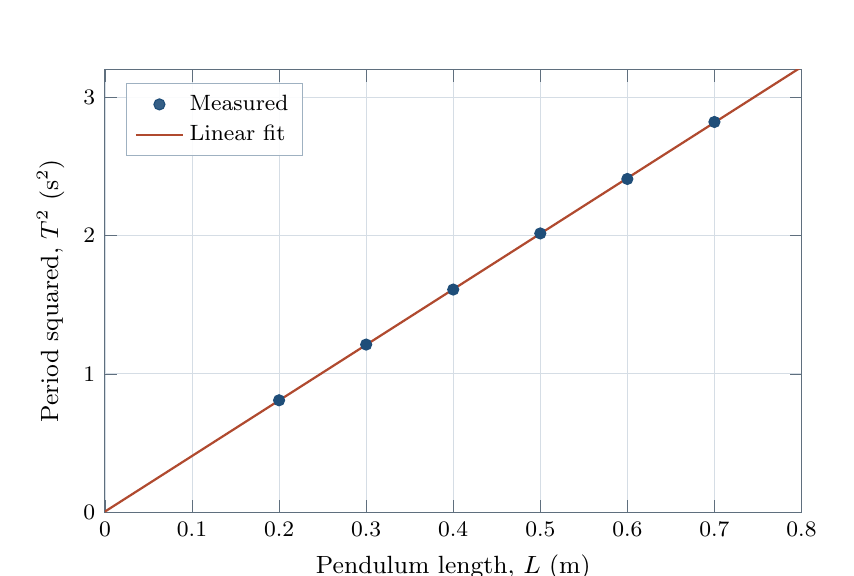
\begin{tikzpicture}
    \begin{axis}[lpaxis, xlabel={Pendulum length, $L$ (\si{\metre})},
                 ylabel={Period squared, $T^{2}$ (\si{\second\squared})},
                 xmin=0, xmax=0.8, ymin=0, ymax=3.2]
      \addplot[only marks, mark=*, mark size=2pt, color=lpAccent,
               error bars/.cd, y dir=both, y explicit] coordinates {
        (0.2,0.809) +- (0,0.003)
        (0.3,1.212) +- (0,0.004)
        (0.4,1.610) +- (0,0.004)
        (0.5,2.016) +- (0,0.005)
        (0.6,2.410) +- (0,0.005)
        (0.7,2.822) +- (0,0.004)
      };
      \addlegendentry{Measured}
      \addplot[domain=0:0.8, samples=2, thick, color=lpAccent2] {4.020*x + 0.004};
      \addlegendentry{Linear fit}
    \end{axis}
  \end{tikzpicture}
  \caption{Period squared versus pendulum length. Error bars show $u(\bar{T}^{2})$ and are smaller than the markers.
           The line is the least-squares fit with slope \SI{4.020}{\second\squared\per\metre}.}
  \label{fig:fit}
\end{figure}

% Example: external image (PDF/PNG) placed in a figures/ folder next to this file.
% \begin{figure}[H]
%   \centering
%   \includegraphics[width=0.8\linewidth]{figures/my-plot.pdf}
%   \caption{Describe what the figure shows, including units and the main trend.}
%   \label{fig:my-plot}
% \end{figure}

% ===== 9. DISCUSSION ===============================================================================================
\section{Discussion}
\ph{Interpret the results. Compare them with theory and the accepted value, explain trends in the plots, and note any
unexpected observations. Refer to tables and figures with Table~\ref{tab:stats} and Figure~\ref{fig:fit}.}

% ===== 10. EXPERIMENTAL UNCERTAINTY AND LIMITATIONS ================================================================
\section{Experimental Uncertainty and Limitations}
Combined standard uncertainty for a result $f(x_1,\dots,x_n)$ with uncorrelated inputs:
\begin{equation}
  u_c(f) = \sqrt{\sum_{i=1}^{n}\left(\frac{\partial f}{\partial x_i}\right)^{2}u^{2}(x_i)} .
  \label{eq:uc}
\end{equation}
Since $g = 4\pi^{2}/m$, this gives $u(g)/g = u(m)/m$.

\begin{table}[H]
  \centering
  \caption{Main sources of uncertainty (sample entries).}
  \label{tab:uncertainty}
  \tblsetup
  \begin{tabular}{@{}p{0.27\linewidth}p{0.15\linewidth}p{0.22\linewidth}p{0.25\linewidth}@{}}
    \toprule\rowcolor{lpTableHead}
    \hdr{Source} & \hdr{Type} & \hdr{Magnitude} & \hdr{Effect on result} \\
    \midrule
    \ph{Length measurement}       & \ph{Systematic} & \ph{\SI{0.001}{\metre}} & \ph{Shifts the $L$ axis} \\
    \ph{Stopwatch resolution}     & \ph{Systematic} & \ph{\SI{0.01}{\second}} & \ph{Small effect on $T$} \\
    \ph{Start/stop reaction time} & \ph{Random}     & \ph{$\approx\SI{0.1}{\second}$} & \ph{Reduced by timing 10 swings} \\
    \ph{Finite amplitude}         & \ph{Systematic} & \ph{$\theta_0\approx 8^{\circ}$} & \ph{Bias in $g$ of about 0.2\%} \\
    \bottomrule
  \end{tabular}
\end{table}

\ph{Discuss limitations of the method, the apparatus and the data set, and how each could be reduced.}

% ===== 11. CONCLUSION ==============================================================================================
\section{Conclusion}
\ph{Restate the objective and the principal result with its uncertainty, say whether the hypothesis or theory was
supported, and suggest one improvement or extension.}

% ===== 12. REFERENCES ==============================================================================================
% REPLACE the sample entries with the sources you cite.
\begin{thebibliography}{9}
  \bibitem{taylor1997} J.~R. Taylor, \emph{An Introduction to Error Analysis: The Study of Uncertainties in Physical
    Measurements}, 2nd ed., University Science Books, 1997.
  \bibitem{gum2008} JCGM~100:2008, \emph{Evaluation of measurement data --- Guide to the expression of uncertainty in
    measurement (GUM)}, BIPM, 2008.
  \bibitem{lab-manual} \ph{Course laboratory manual: title, author, edition, year.}
\end{thebibliography}

% ===== 13. APPENDICES (OPTIONAL) ===================================================================================
% Delete everything from \appendix onward if the report does not need appendices.
\appendix
\section{Raw Data and Instrument Details}
\ph{Include complete data logs, calibration records and instrument specifications that would interrupt the main text.}

\section{Supplementary Derivations}
\ph{Add extended derivations, additional calculations or code listings here.}

\end{document}
